\documentclass[10pt,a4paper]{article}
\usepackage[portuguese, english]{babel}
\usepackage[utf8]{inputenc}
\usepackage{graphicx}
\usepackage{amsmath,amsfonts}
\usepackage{setspace}
%documentclass[twocolumn]{article}
\usepackage{multicol}
\usepackage{indentfirst}
\usepackage[margin=1.3cm]{geometry}
\usepackage{pst-circ}
\usepackage{supertabular}
\usepackage{url}                         % Gestão de links no pdf
\usepackage[]{epstopdf}                  % Inclusão de imagens .eps
\usepackage{mdframed}

\input epsf

\hyphenation{asso-ciada}

\begin{document}
\twocolumn[
\centerline{\Large \textbf{Problema da Conectividade}}
\centerline{\textbf{Análise da implementação de algoritmos em linguagem C}}
\vskip 0.3cm
\centerline{Laboratórios de Algoritmos e Estruturas de Dados}
\vskip 0.3cm
\centerline{Grupo X - 2ªfeira}
\centerline{Beatriz Ferreira 78794; Henrique Nogueira 78927}
\centerline{Professor -------}
\vskip 0.5cm
\centerline{21 de Setembro de 2016}
\vskip 0.5cm

%-------------------------------------------------------------
\centerline{
\parbox[0]{0.8\textwidth}{
\textbf{Resumo: }Perante o problema da Conectividade, foi feita uma análise da eficácia de resolução para 4 Algoritmos distintos para diferentes níveis de complexidade do problema. }}
\vskip 1.2 cm
]
%-------------------------------------------------------------


%---------------------INTROCUÇÃO---------------------------------------


\section{Introdução e Motivaç\~ao}

\par Dado um número \textbf{N} de objectos, cada um identificado por um inteiro, e uma sequência com pares de objectos (\textbf{p-q}), representando uma ligação entre si, o \textbf{problema da Conectividade} consiste em saber se, dado um par de objectos arbitrários, existe uma ligação entre ambos, directa ou indirectamente. 
\par Este problema tem interesse em ser estudado pois objectos abstractos podem ser traduzidos em objectos reais, permitindo a resolução de problemas do mundo real, como por exemplo:
\begin{itemize}
\item numa rede de computadores, saber se um está ligado a outro
\item saber se dois pontos de contacto de um circuito estão ligados entre si
\item saber se existe uma ligação directa ou indirecta entre duas pessoas numa rede social
\end{itemize}
\par É portanto vital saber que Algoritmo implementar pois, dependendo do grau de complexidade do problema, a eficácia de resolução pode ser melhorada em várias ordens de grandeza permitindo tomar maior partido do poder de computação de uma dada máquina.

\section{Implementaç\~ao dos Algoritmos}

\par Em laboratório,foi feita uma análise da eficácia de diferentes Algoritmos para diferentes níveis de complexidade diferente. Para este efeito foram implementados 4 Algoritmos diferentes.
\par Visto que para a resolução deste problema não é necessário saber o caminho percorrido que liga dois objectos mas apenas se estes estão de facto ligados, basta-nos distribuir os objectos por diferentes conjuntos, representando objectos ligados, e ir aglomerando á medida que é recebida informação acerca das ligações entre si, perdendo no processo informação relativa á ordem de ligação. Podemos portanto dividir este processo em 2 fases distintas, a Procura (\textbf{Find}), onde se identifica se dois objectos estão contidos num mesmo conjunto, e a União (\textbf{Union}) onde se faz a junção de dois conjuntos distintos. O fluxograma representado na \textbf{figura 1} exprime precisamente este processo:
\begin{enumerate}
\item é lido um par de objectos vindo da sequência de pares
\item a procura obtém o identificador de conjunto de cada objecto
\item o identificador exprime a coexistência dos objectos no mesmo conjunto, permitindo saber se \textbf{p} e \textbf{q} se encontram ligados
\item \textbf{caso não se encontrem ligados} segue-se o processo de União onde se quer igualar os identificadores de cada objecto de ambos os conjuntos
\end{enumerate}
\begin{figure}[h!]
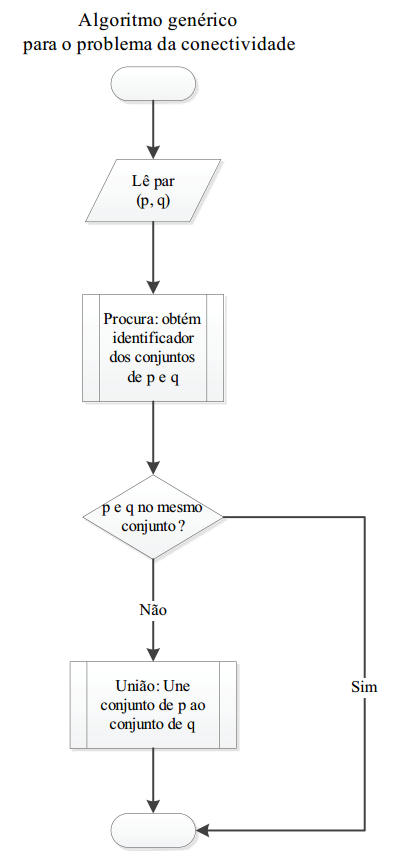
\includegraphics[scale=0.5]{fluxo1.png}
\caption{Fluxograma genérico de um algoritmo de resolução do problema da conectividade (por aglomeração de conjuntos)}
\end{figure}
\par Para cada um dos algoritmos que se seguem é usada a mesma estrutura de dados, uma tabela de identificadores \textbf{id} cujo índice representa o objecto.

\subsection{QF - Algoritmo de Procura rápida}
\par O primeiro algoritmo a analisar é o algoritmo de procura rápida, que como o nome indica tem uma fase de procura mais rápida, necessitando apenas de uma operação para concretizar a verificação. A ideia é que o identificador do conjunto está imediatamente contido na identificador da tabela, isto é, se \textbf{p} e \textbf{q} estão contidos num mesmo conjunto então \textbf{id[p]=id[q]}.
\par Em contrapartida de uma operação de procura rápida, a sua união é mais lenta pois implica que para cada união de conjuntos é necessário percorrer a tabela inteira e redefenir o identificador de todos os objectos que pertenciam a um desses conjuntos.
\begin{figure}[h!]
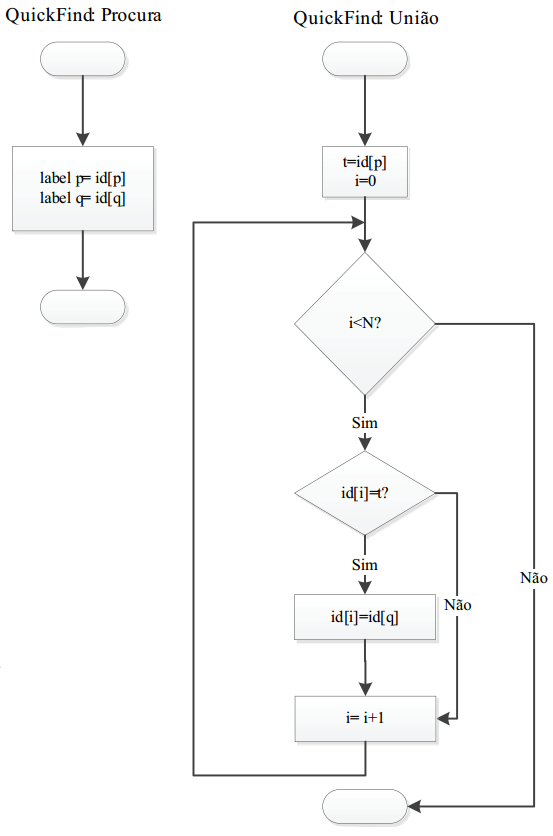
\includegraphics[scale=0.5]{flux2.png}
\caption{Operações de procura e união de algoritmo Quick-Find. A operação de procura é executada num só passo inquirindo se id[q]=id[p]. A operação de união já exige a leitura e actualização de todos os identificadores antigos da tabela.}
\end{figure}
\par Podemos dizer com certeza que o número de operações de procura é sempre igual a \textbf{M}, número de pares, pois para cada novo par a procura é feita num só inquérito (\textbf{id[q]==id[p]})
\par Quanto á união é mais incerto pois este dependerá do número de ligações, \textbf{L}, pois caso o resultado da procura seja positiva não haverá união por fazer. Podemos no entanto garantir que pelo menos \textbf{(N+1)L} operações de união são feitas pois para cada ligação a tabela é lida N vezes e escrita pelo menos 1 vez.
\par No entanto, para \textbf{M$>>$N} com \textbf{N$>>$1}, temos na maior parte dos casos \textbf{L} na mesma ordem de grandeza de \textbf{N}, pois o número máximo de ligações é no máximo (\textbf{N-1}), e portanto o número de operações expectável é aproximadamente \textbf{N}$^2$. Finalmente este algoritmo também tem a propriedade de aumentar em velocidade assim que a união entre todos os pontos fica estabelecida pois o processo de união nunca mais é chamado.

\subsection{QU - Algoritmo de União Rápida}
\par Este algoritmo por sua vez tem um processo de uni\~ao rápida em contrapartida com um processo de procura mais lenta. A ideia desta vez está em vez em estabelecer uma hierarquia de ponteiros que convirjam numa raíz do conjunto, isto é, se a procura indicar uma nova ligação entre \textbf{p} e \textbf{q} faz-se \textbf{id[p]=q} estabelecendo a ligação ao apontar arbritáriamente \textbf{p} á raíz de \textbf{q}. Desta forma cria-se uma estrutura de conjuntos em forma de árvore cujo cada elemento aponta para o próximo até chegar á raíz que por sua vez aponta para si mesma. Percebe-se portanto que o número de operações de procura é superior pois o identificador de conjunto está "escondido" a cada objecto, sendo necessário seguir o caminho de ponteiros para o encontrar.
\par O processo de união é sempre feito numa operação dada uma nova ligação, pelo que no total é feita em \textbf{L} operações.
\par Por sua vez, o número de operações de procura é incerto pois o número de procuras por par dependerá da estrutura de árvore dos conjuntos em causa. No entanto para valores de \textbf{N} pequenos iremos ter uma estrutura de árvores mais favorável a uma procura mais rápida pois para cada procura temos que seguir no máximo uma cadeia de \textbf{N} objectos, pelo que teóricamente será mais eficaz nesses casos. Em oposição ao Algoritmo de União rápida, este Algoritmo continua a demorar o mesmo tempo de execução mesmo após estabelecida a ligação entre os pontos.

\subsection{WQU - Algoritmo de Uni\~ao Rápida equilibrada}
\par Este algoritmo é equivalente ao algoritmo anterior de uma maneira geral, excepto que em vez de ser feita arbitráriamente a estrutura em árvore dos conjuntos, escolhe-se sempre apontar o objecto com o menor conjunto em árvore da qual ele é raíz, permitindo uma melhor distribuição dos nodos da árvore e por sua vez diminuindo a quantidade de ponteiros a seguir para chegar á raíz do conjunto aglomerado. No entanto, a memória gasta é duplicada já que é necessário acrescentar uma tabela com os tamanhos dos conjuntos correspondentes bem como acrescentar ás operações de união os passos relativos á actualização desta nova tabela.
\par É possível provar\footnote{Ref. Algorithms in C, Robert Sedgewick} que para cada processo de procura cada objecto tem de seguir no máximo \textbf{Log(N)} ponteiros até chegar á raíz, pelo que as operações de procura não devem exceder \textbf{MLog(N)} operações.
\par Já as operações de união são no máximo 3 por par: leitura e comparação de tamanhos, associação de ponteiro e por fim update da tabela de tamanhos.

\subsection{CWQU - Algoritmo de Uni\~ao Rápida equilibrada comprimida}
\par Semelhante ao Algoritmo de Uni\~ao Rápida equilibrada, este por sua vez acrescenta mais ao processo de uni\~ao fazendo ligar todos os objectos que procedem o ponteiro inicial directamente á raíz do seu objecto par.
\par Torna-se óbvio que para \textbf{M} e \textbf{N} grandes este processo díminui considerávelmente o número de operações de procura necessárias, no entanto para \textbf{N} e \textbf{M} muito pequenos poderá representar trabalho desnecessário.

%--------------------Montagem e procedimento-------------------------------


\section{Resultados experimentais}
\par Para colocar os Algoritmos á prova foi necessário contabilizar o número de operações de procura e união efectuadas por cada um para problemas de diferente complexidade. Utilizou-se para esse efeito o programa fornecido, juntamente com os dados, ao qual apenas foi necessário implementar os contadores necessários.
\par \textbf{f\_cnt} e \textbf{u\_cnt} são respectivamente os contadores de operações de procura e de união aos quais se vai incrementar sucessivamente o valor para uma operação de leitura ou actualização da tabela.
\par A tabela 1 apresenta o resultado obtido correndo cada Algoritmo com 9 configurações de pares, \textbf{N}, \textbf{M} e \textbf{L}.

\begin{table}[h!]
\centering
\resizebox{\columnwidth}{!}{%
\begin{tabular}{llll|l|l|l|l|}
\cline{5-8}
                                &                             &                              &          & \multicolumn{2}{l|}{{\bf Quick Find}} & \multicolumn{2}{l|}{{\bf Quick Union}} \\ \hline
\multicolumn{1}{|l|}{Dados}     & \multicolumn{1}{l|}{Nós}    & \multicolumn{1}{l|}{Pares}   & Ligações & Find            & Union               & Find                  & Union          \\ \hline
\multicolumn{1}{|l|}{10.txt}    & \multicolumn{1}{l|}{10}     & \multicolumn{1}{l|}{5}       & 4        & 5               & 47                  & 8                     & 5              \\ \hline
\multicolumn{1}{|l|}{100.txt}   & \multicolumn{1}{l|}{100}    & \multicolumn{1}{l|}{200}     & 49       & 200             & 5,340               & 2,910                 & 200            \\ \hline
\multicolumn{1}{|l|}{1000.txt}  & \multicolumn{1}{l|}{1,000}  & \multicolumn{1}{l|}{2,000}   & 499      & 2,000           & 531,892             & 185,503               & 2,000          \\ \hline
\multicolumn{1}{|l|}{10000.txt} & \multicolumn{1}{l|}{10,000} & \multicolumn{1}{l|}{20,000}  & 4,998    & 20,000          & 53,232,431          & 18,479,087            & 20,000         \\ \hline
\multicolumn{1}{|l|}{a.txt}     & \multicolumn{1}{l|}{1,000}  & \multicolumn{1}{l|}{6,206}   & 999      & 6,206           & 1,120,579           & 1,211,723             & 6,206          \\ \hline
\multicolumn{1}{|l|}{b.txt}     & \multicolumn{1}{l|}{2,500}  & \multicolumn{1}{l|}{20,236}  & 2,499    & 20,236          & 7,013,153           & 10,603,943            & 20,236         \\ \hline
\multicolumn{1}{|l|}{c.txt}     & \multicolumn{1}{l|}{5,000}  & \multicolumn{1}{l|}{41,913}  & 4,999    & 41,913          & 28,182,683          & 45,839,698            & 41,913         \\ \hline
\multicolumn{1}{|l|}{d.txt}     & \multicolumn{1}{l|}{10,000} & \multicolumn{1}{l|}{83,857}  & 9,999    & 83,857          & 112,960,455         & 186,599,079           & 83,857         \\ \hline
\multicolumn{1}{|l|}{e.txt}     & \multicolumn{1}{l|}{25,000} & \multicolumn{1}{l|}{309,802} & 24,999   & 309,802         & 704,627,920         & 1,782,620,002         & 309,802        \\ \hline
\end{tabular}
}
\end{table}
\begin{table}[h!]
\centering
\resizebox{\columnwidth}{!}{%
\begin{tabular}{llll|l|l|l|l|}
\cline{5-8}
                                &                             &                              &          & \multicolumn{2}{l|}{{\bf Weighted Quick Union}} & \multicolumn{2}{l|}{{\bf Compressed WQU }} \\ \hline
\multicolumn{1}{|l|}{Dados}     & \multicolumn{1}{l|}{Nós}    & \multicolumn{1}{l|}{Pares}   & Ligações & Find                     & Union                & Find          & Union       \\ \hline
\multicolumn{1}{|l|}{10.txt}    & \multicolumn{1}{l|}{10}     & \multicolumn{1}{l|}{5}       & 4        & 18                       & 12                   & 15            & 13          \\ \hline
\multicolumn{1}{|l|}{100.txt}   & \multicolumn{1}{l|}{100}    & \multicolumn{1}{l|}{200}     & 49       & 1,119                    & 147                  & 595           & 195         \\ \hline
\multicolumn{1}{|l|}{1000.txt}  & \multicolumn{1}{l|}{1,000}  & \multicolumn{1}{l|}{2,000}   & 499      & 12,074                   & 1,497                & 6,620         & 2,002       \\ \hline
\multicolumn{1}{|l|}{10000.txt} & \multicolumn{1}{l|}{10,000} & \multicolumn{1}{l|}{20,000}  & 4,998    & 127,290                  & 14,994               & 66,693        & 20,253      \\ \hline
\multicolumn{1}{|l|}{a.txt}     & \multicolumn{1}{l|}{1,000}  & \multicolumn{1}{l|}{6,206}   & 999      & 40,067                   & 2,997                & 22,058        & 4,009       \\ \hline
\multicolumn{1}{|l|}{b.txt}     & \multicolumn{1}{l|}{2,500}  & \multicolumn{1}{l|}{20,236}  & 2,499    & 131,737                  & 7,497                & 71,116        & 10,087      \\ \hline
\multicolumn{1}{|l|}{c.txt}     & \multicolumn{1}{l|}{5,000}  & \multicolumn{1}{l|}{41,913}  & 4,999    & 275,402                  & 14,997               & 148,030       & 20,198      \\ \hline
\multicolumn{1}{|l|}{d.txt}     & \multicolumn{1}{l|}{10,000} & \multicolumn{1}{l|}{83,857}  & 9,999    & 565,155                  & 29,997               & 298,584       & 40,616      \\ \hline
\multicolumn{1}{|l|}{e.txt}     & \multicolumn{1}{l|}{25,000} & \multicolumn{1}{l|}{309,802} & 24,999   & 2,139,355                & 74,997               & 1,116,831     & 101,506     \\ \hline
\end{tabular}
}
\caption{Tabelas de resultados experimentais}
\label{my-label}
\end{table}


%----------------------Analise de resultados--------------------------

\section{Análise de resultados}
\par Numa análise superficial, é vísivel que os algoritmos \textbf{QF} e \textbf{QU}, embora a um nível de eficácia comparável para graus de complexidade muito baixos, assim que se aumenta a dificuldade o número de operações explode. Isto indica desde logo que ambos os algoritmos reajem não linearmente com \textbf{N}. Em oposição, \textbf{WQU} e \textbf{CWQU} apresentam um comportamento mais linear, sendo observável que por cada ordem de grandeza de \textbf{N} o número de operações aumenta também aproximadamente em uma ordem de grandeza, indicando comportamento aproximadamente linear com \textbf{N}.
\subsection{QF - análise de resultados}
\par Fazendo um gráfico de dispersão logarítmico para o número de operações de união (\textbf{U}) podemos investigar se há uma relação exponêncial com \textbf{N}.

%Introduzir Gráfico Ln(U)(Ln(N))
\begin{figure}[h!]
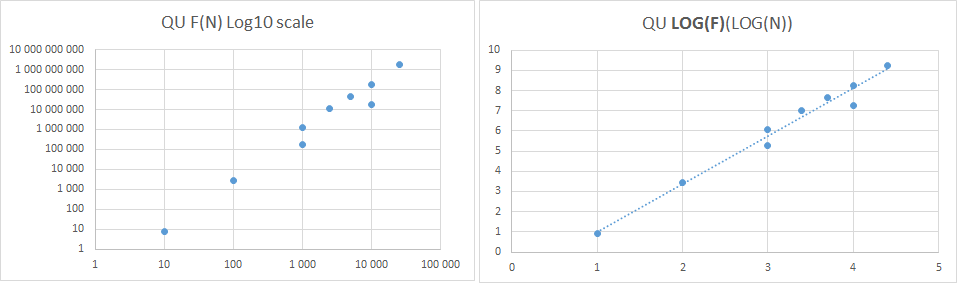
\includegraphics[scale=0.35]{QUgraphs.png}
\caption{QF - Á esquerda: plot de U(N) em escala logarítmica; á direita: regressão linear sobre \textbf{Ln(U)}(Ln(N)) }
\end{figure}
\par Observando os gráficos da figura 3, com excepção de dois dos pontos experimentais obtidos, podemos concluir que a regressão linear foi correctamente aplicadamente aplicada ao gráfico devolvendo um declive de 2. Temos portanto uma verificação do comportamento previsto de que \textbf{U$\simeq$N}$^2$.
\par Como expectável, o número de operações de procura é igual a \textbf{M}, não sendo necessária fazer uma análise gráfica sobre \textbf{F}.

\subsection{QU - análise de resultados}
\par Repetindo o mesmo processo da análise imediatamente anterior...

%Introduzir Gráfico
\begin{figure}[h!]
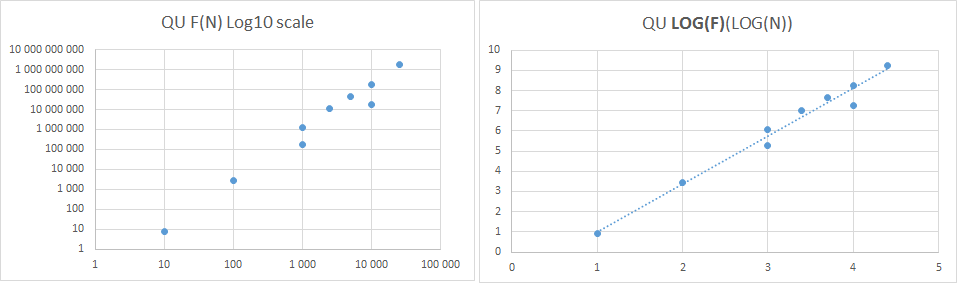
\includegraphics[scale=0.4]{QUgraphs.png}
\caption{QU - Á esquerda: plot de F(N) em escala logarítmica; á direita: regressão linear sobre \textbf{Ln(F)}(Ln(N)) }
\end{figure}
\par Paralelamente ao primeiro algoritmo, a regressão linear realizada sobre o plot logaritmico de \textbf{F(N)} devolve um declive de 2, podendo também ser feita a conclusão \textbf{F(N)=N$^2$}.
\par O número de operações de união está exactamente de acordo com o previsto.
\par Por fim á que acrescentar que o número de operações deste algoritmo é superior ao algoritmo \textbf{QF} para valores de \textbf{N} muito grandes, e mais especificamente \textbf{M $>>$ N}. Uma razão mais óbvia para que tal aconteça é pois, mesmo quando as ligações entre todos os objectos já estão estabelecidas, que se pode confirmar ser o caso devido a \textbf{L=N-1}, este algoritmo continua a ter o mesmo número de operações para cada novo par enquanto \textbf{QF} apenas verifica a já existente ligação.

\subsection{WQU e CWQU - análise de resultados}
\par Por fim, ambos os algoritmos \textbf{WQU} e \textbf{CWQU} provaram ser verdadeiramente eficazes para todos os graus de complexidade testados. Fazendo os respectivos gráficos de dispersão obtivemos as imagens da figuras 5 e 6.

\begin{figure}[h!]
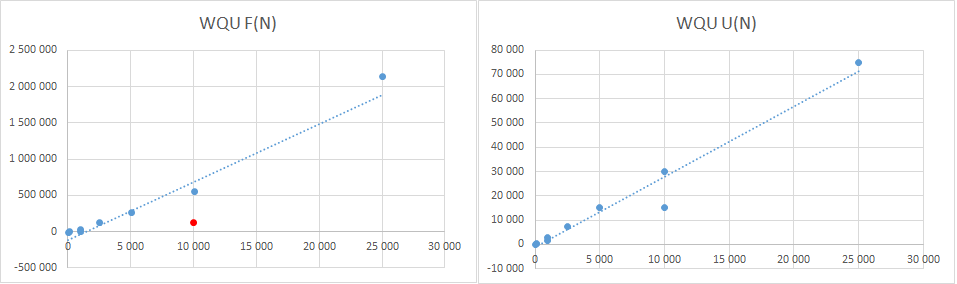
\includegraphics[scale=0.35]{WQUgraphs.png}
\caption{WQU - Á esquerda: regressão linear do plot de F(N) ; á direita: regressão linear do plot U(N) }
\end{figure}

\begin{figure}[h!]
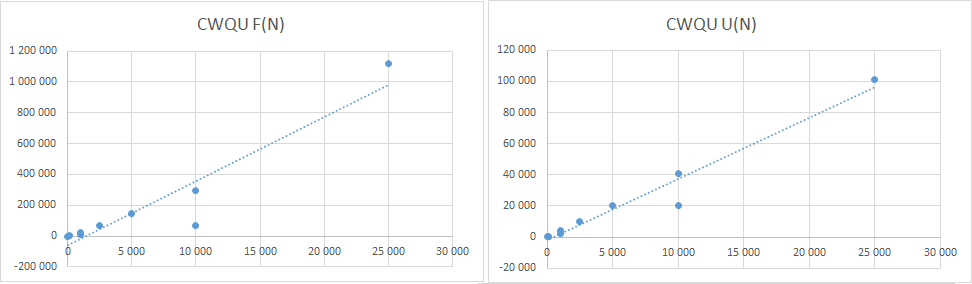
\includegraphics[scale=0.35]{CWQUgraphs.png}
\caption{CWQU - Á esquerda: regressão linear do plot de F(N); á direita: regressão linear do plot F(N) }
\end{figure}

\par Embora a amostra de resultados não seja suficiente, a regressão linear destes gráficos de dispersão parece que foi bem sucedida a menos de um dos pontos. 
\par Para o algoritmo \textbf{WQU} obtivemos o valor de declive representando \textbf{F(N)$\simeq$60N} e \textbf{U(N)$\simeq$3N} e para \textbf{CWQU} os respectivos valores \textbf{F(N)$\simeq$40N} e \textbf{U(N)$\simeq$4N}, verificando-se assim uma maior eficácia na procura por parte de \textbf{CWQU} ao custo de uma ligeiro aumento no tempo de união e compressão.

%------------------CONCLUSÃO-------------------------

\section{Análise crítica e Conclusão}

\par Após a análise dos resultados experimentais podemos concluir que estes estavam de acordo com os valores esperados. O algoritmo \textbf{CWQU} deve ser portanto implementado para uma aplicação usual do problema da conectividade, tendo no entanto em conta que para valores baixos na ordem de \textbf{N=10} este fica atrás de \textbf{QU} (28 operações totais contra apenas 13), devido a uma maior complexidade nas operações de compressão e equilibrio associadas. No entanto, com alguma surpresa, verifica-se que se pode esperar uma resposta que aumenta aproximadamente linearmente com o aumento de \textbf{N} tanto para \textbf{WQU} como \textbf{CWQU}. 
\par Quanto aos algoritmos \textbf{QU} e \textbf{QF}, podemos esperar na maior parte dos casos um tempo quadrático em ordem ao número de objectos.
\par No entanto, é importante acrescentar que o comportamento destes algoritmos pode ser imprevisivel, como se pode inferir dos dados \textbf{1000.txt} e \textbf{10000.txt} que estavam claramente fora das linhas obtidas por regressão linear. Portanto na aplicação destes algoritmos deve-se ter tido em conta a aleatoriadade ou não da forma como estão distribuidas as ligações.

\section{Extra - Impressão dos conjuntos na função de Algoritmo Quick-Find}
\par Por fim, no ponto 4 do enunciado é pedida a implementação de código que imprima dos diferentes conjuntos obtidos. Para tal o código segue as seguintes instruções:

\begin{enumerate}
\item O número de conjuntos diferentes é dado por \textbf{N-L=set\_cnt}
\item Usar codificação: \textbf{id[i]==-1$\Rightarrow$ já foi impresso}
\item Encontrar o primeiro \textbf{id[i]!=-1} e guardar o conjunto a ser impresso numa variável (\textbf{t}
\item Imprimir todos os objectos com \textbf{id[i]==t}
\item Repetir o processo \textbf{set\_cnt} vezes até imprimir todos os objectos
\end{enumerate}




%-------------------------------------------------------------
\vskip 10cm
\section{Referências}
\begin{itemize}
\item Algorithms in C, Robert Sedgewick
\item Aulas teóricas, Prof. Carlos Bispo; Instituto Superior Técnico, Departamento de Engenharia Electrotécnica e de Computadores
\end{itemize}
\end{document}
